\chapter{Módulo: Pacientes y Profesionales}
\label{mod:02-pacientes-y-profesionales}

\section{Propósito}
\label{sec:pacientes-proposito}

Administra las dos bases de personas que participan directamente de la atención clínica: los pacientes de la óptica y los profesionales de salud (optómetras/oftalmólogos) que los atienden. Ambos parten de \code{Person}, pero con reglas de acceso opuestas: el paciente puede existir sin cuenta, el profesional siempre la necesita.

\section{Entidades principales}
\label{sec:pacientes-entidades}

Ver Capítulo~\ref{sec:modelo-datos} para el diagrama completo.

\begin{longtable}{p{3.4cm}p{10cm}}
\caption{Entidades principales del módulo de Pacientes y Profesionales.}\label{tab:pacientes-entidades}\\
\toprule
\textbf{Entidad} & \textbf{Rol} \\
\midrule
\endfirsthead
\toprule
\textbf{Entidad} & \textbf{Rol} \\
\midrule
\endhead
\bottomrule
\endfoot
\code{Patient} & Marca que una \code{Person} es paciente. \code{UserId} \textbf{nullable} --- puede existir sin acceso al sistema. \\
\code{Professional} & Marca que una \code{Person} es profesional de salud. \code{UserId} \textbf{obligatorio} (1:1). \\
\code{Especialidad} / \code{Profesional}\allowbreak \code{Especialidad} & Catálogo de especialidades, many-to-many con \code{Professional}. \\
\code{Horario}\allowbreak \code{Profesional} / \code{PausaHorario} / \code{BloqueoFecha} & Disponibilidad del profesional --- consumida por el módulo Agenda, se gestiona desde aquí (formulario de Profesional). \\
\end{longtable}

\section{Reglas de negocio clave}
\label{sec:pacientes-reglas}

\begin{itemize}
  \item \textbf{Paciente sin cuenta es el caso normal, no la excepción:} recepción da de alta un paciente con solo CI/nombre/contacto (\code{Patient.UserId = null}). Solo si el paciente necesita el portal de autogestión (ver sus turnos/recetas/historial) se crea un \code{User} vinculado --- vía el flujo de auto-registro público, no desde el ABM interno de pacientes. Ver Capítulo~\ref{mod:01-identidad-y-acceso}.
  \item \textbf{Profesional siempre requiere \code{User}} --- no existe un ``profesional sin login''. El alta de un profesional crea \code{Person}+\code{User}+\code{Professional} en una sola operación transaccional, con \code{Is}\allowbreak \code{Email}\allowbreak \code{Verified=true} e \code{Is}\allowbreak \code{User}\allowbreak \code{Must}\allowbreak \code{Change}\allowbreak \code{Password=true} (cuenta vouched-for por el admin, no auto-registro).
  \item \textbf{La sucursal del profesional se asigna en este formulario, no en \code{UsuariosView}} --- es una decisión explícita del rediseño multi-sucursal (2026-06-28): \code{User.SucursalId} se sigue guardando en \code{User}, pero la UX de asignación vive en \code{ProfesionalesView}/\code{EmpleadosView}, no en la pantalla de usuarios (que solo gestiona roles y activar/desactivar).
  \item \textbf{Un profesional puede tener más de una especialidad} (many-to-many vía \code{Profesional}\allowbreak \code{Especialidad}), a diferencia de un diseño más simple de ``una especialidad por profesional''.
  \item \textbf{Disponibilidad del profesional es multi-capa:} \code{Horario}\allowbreak \code{Profesional} (horario semanal recurrente, por sucursal --- índice único \code{Professional}\allowbreak \code{Id+Sucursal}\allowbreak \code{Id+Dia}\allowbreak \code{Semana}), \code{PausaHorario} (recesos dentro de un horario, ej.\ almuerzo) y \code{BloqueoFecha} (excepciones puntuales, ej.\ vacaciones). Los tres alimentan el cálculo de slots disponibles del módulo Agenda, pero se gestionan desde el form de Profesional.
  \item \textbf{Borrado lógico} (\code{Patient.IsActive} / desactivación de \code{User} para \code{Professional}) --- sin borrado físico.
\end{itemize}

\section{Endpoints}
\label{sec:pacientes-endpoints}

Detalle completo en el Apéndice de Referencia de API (\code{Patients}\allowbreak \code{Controller}, \code{Professionals}\allowbreak \code{Controller}, \code{Especialidades}\allowbreak \code{Controller}, \code{Horarios}\allowbreak \code{Controller} anidado bajo \code{/}\allowbreak \code{api/}\allowbreak \code{professionals/}\allowbreak \code{{id}}).

\begin{longtable}{p{6.4cm}p{7cm}}
\caption{Endpoints principales del módulo de Pacientes y Profesionales.}\label{tab:pacientes-endpoints}\\
\toprule
\textbf{Método} / \textbf{Ruta} & \textbf{Descripción} \\
\midrule
\endfirsthead
\toprule
\textbf{Método} / \textbf{Ruta} & \textbf{Descripción} \\
\midrule
\endhead
\bottomrule
\endfoot
GET/\allowbreak POST/\allowbreak PUT/\allowbreak DELETE\code{/api/patients} & CRUD más desactivación de pacientes. \\
GET/\allowbreak POST/\allowbreak PUT/\allowbreak DELETE\code{/}\allowbreak \code{api/}\allowbreak \code{professionals} & CRUD más desactivación de profesionales. \\
GET/\allowbreak POST/\allowbreak PUT/\allowbreak DELETE\code{/}\allowbreak \code{api/}\allowbreak \code{especialidades} & Catálogo de especialidades. \\
GET/PUT \code{/}\allowbreak \code{api/}\allowbreak \code{professionals/}\allowbreak \code{{id}/horarios} & Horario semanal (reemplaza el set completo por sucursal). \\
GET/POST/DELETE \code{/}\allowbreak \code{api/}\allowbreak \code{professionals/}\allowbreak \code{{id}/bloqueos} & Fechas bloqueadas. \\
\end{longtable}

\section{Flujo típico}
\label{sec:pacientes-flujo}

\subsection{Alta de profesional (transacción multi-entidad)}

\begin{figure}[htbp]
\centering
\begin{tikzpicture}
  \node[actor] (fe) at (0,0) {SIGA-Web\\\footnotesize ProfesionalesView};
  \node[actor] (api) at (4,0) {Professionals\\Controller};
  \node[actor] (svc) at (8,0) {Professional\\Service};
  \node[actor] (db) at (12,0) {PostgreSQL};

  \draw[lineavida] (fe.south) -- ++(0,-8.3);
  \draw[lineavida] (api.south) -- ++(0,-8.3);
  \draw[lineavida] (svc.south) -- ++(0,-8.3);
  \draw[lineavida] (db.south) -- ++(0,-8.3);

  \draw[mensaje] ($(fe.south)+(0,-1.0)$) -- node[above,font=\scriptsize,align=center]{POST /professionals\\(datos + specialty + sucursalId)} ($(api.south)+(0,-1.0)$);
  \draw[mensaje] ($(api.south)+(0,-2.2)$) -- node[above,font=\scriptsize]{CreateAsync(request)} ($(svc.south)+(0,-2.2)$);
  \draw[mensaje] ($(svc.south)+(0,-3.1)$) -- node[above,font=\scriptsize]{crea Person} ($(db.south)+(0,-3.1)$);
  \draw[mensaje] ($(svc.south)+(0,-4.2)$) -- node[above,font=\scriptsize,align=center]{crea User (SucursalId,\\IsEmailVerified=true, MustChangePassword=true)} ($(db.south)+(0,-4.2)$);
  \draw[mensaje] ($(svc.south)+(0,-5.3)$) -- node[above,font=\scriptsize]{crea Professional (UserId, LicenseNumber)} ($(db.south)+(0,-5.3)$);
  \draw[mensaje] ($(svc.south)+(0,-6.1)$) -- node[above,font=\scriptsize]{asigna rol ``Professional'' (UserRole)} ($(db.south)+(0,-6.1)$);
  \draw[mensaje] ($(svc.south)+(0,-7.2)$) -- node[above,font=\scriptsize,align=center]{crea ProfesionalEspecialidad\\por cada especialidad elegida} ($(db.south)+(0,-7.2)$);
  \draw[mensajeretorno] ($(api.south)+(0,-7.9)$) -- node[below,font=\scriptsize]{200 OK} ($(fe.south)+(0,-7.9)$);
\end{tikzpicture}
\caption{Alta de profesional: transacción única que crea \texttt{Person}, \texttt{User}, \texttt{Professional}, asigna el rol y las especialidades.}
\label{fig:seq-alta-profesional}
\end{figure}

\subsection{Alta de paciente sin cuenta (caso normal)}

Recepción completa un formulario simple (CI/nombre/contacto) $\to$ \code{POST /api/patients} crea \code{Person}+\code{Patient} sin \code{User}. El paciente queda disponible de inmediato para agendar turnos, tener historia clínica y figurar en ventas --- no hace falta que tenga acceso al portal.

\section{Vistas de frontend}
\label{sec:pacientes-vistas}

\begin{itemize}
  \item \code{PacientesView.vue}, \code{PacienteNuevoView.}\allowbreak \code{vue}, \code{PacienteDetailView.}\allowbreak \code{vue}
  \item \code{ProfesionalesView.}\allowbreak \code{vue} (incluye asignación de sucursal, horarios y especialidades)
  \item \code{EspecialidadesView.}\allowbreak \code{vue}
  \item Portal del paciente (autogestión, requiere \code{Patient.UserId} no nulo): \code{MiHistorialView.}\allowbreak \code{vue}, \code{MisRecetasView.}\allowbreak \code{vue} --- documentadas en detalle en el \hyperref[mod:05-clinica]{Módulo de Clínica}, ya que son vistas de historial clínico, no de datos personales.
\end{itemize}

\section{Interfaz}
\label{sec:pacientes-interfaz}

\begin{figure}[htbp]
\centering
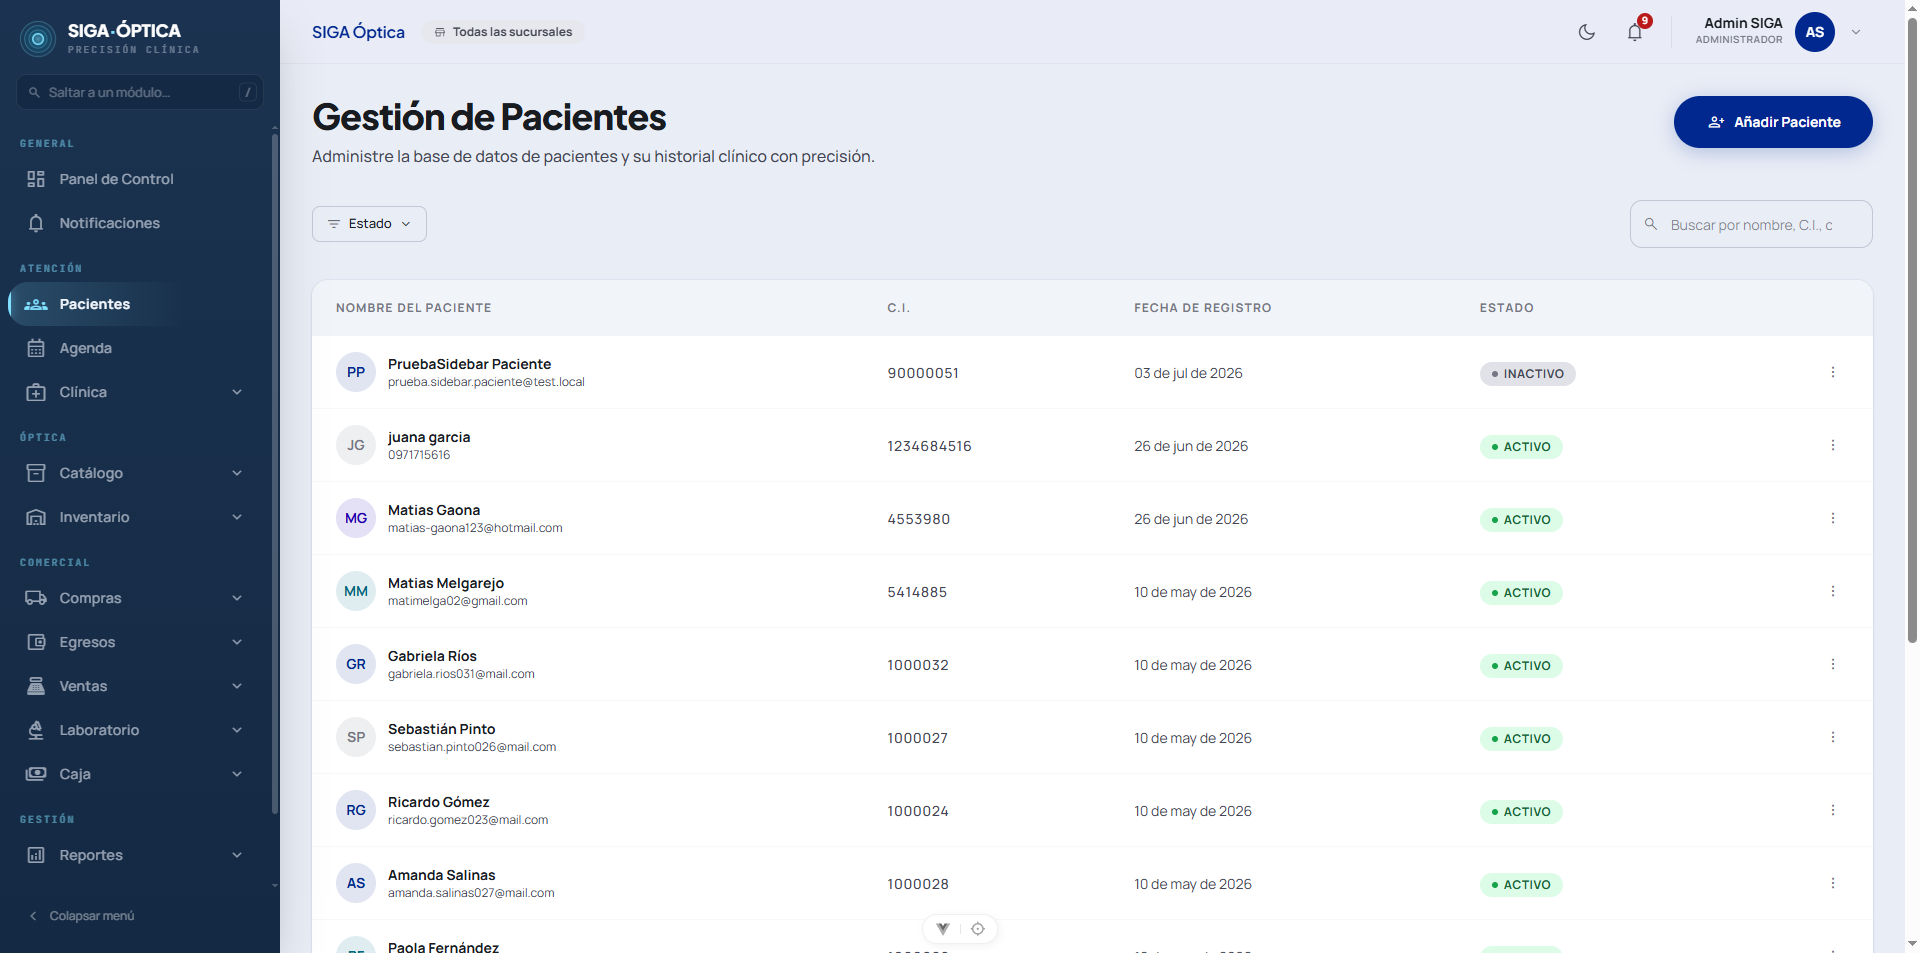
\includegraphics[width=0.95\textwidth]{imagenes/mod02-pacientes.png}
\caption{Listado de pacientes registrados en el sistema.}
\label{fig:mod02-pacientes}
\end{figure}

\section{Estado}
\label{sec:pacientes-estado}

\Implementado. Sin limitaciones conocidas relevantes para la tesis más allá de las ya anotadas en el Apéndice de Referencia de API (ej.\ \code{DELETE /api/professionals/{id}} usa la policy \code{editar_}\allowbreak \code{profesional} en vez de una policy de desactivación dedicada, a diferencia de \code{Patient}/\code{Cliente}).
